\subsubsection{Information}
\begin{itemize}
	\item \textbf{Course Name:} \href{https://www.coursera.org/learn/responsive-web-design-adobe-xd}{Build Dynamic User Interfaces (UI) for Websites}
	\item \textbf{Instructor:} \href{https://www.coursera.org/instructor/google-career-certificates}{Google Career Certificates}
	\item \textbf{Level:} Beginner
	\item \textbf{Enrolled on:} July 6, 2024
	\item \textbf{Finished on:} July 29, 2024
	\item \textbf{Grade Achieved:} 90.00\%
\end{itemize}

\subsubsection{Course is done}
\begin{figure}[!ht]
	\centering
	\begin{subfigure}{0.75\textwidth}
		\centering
		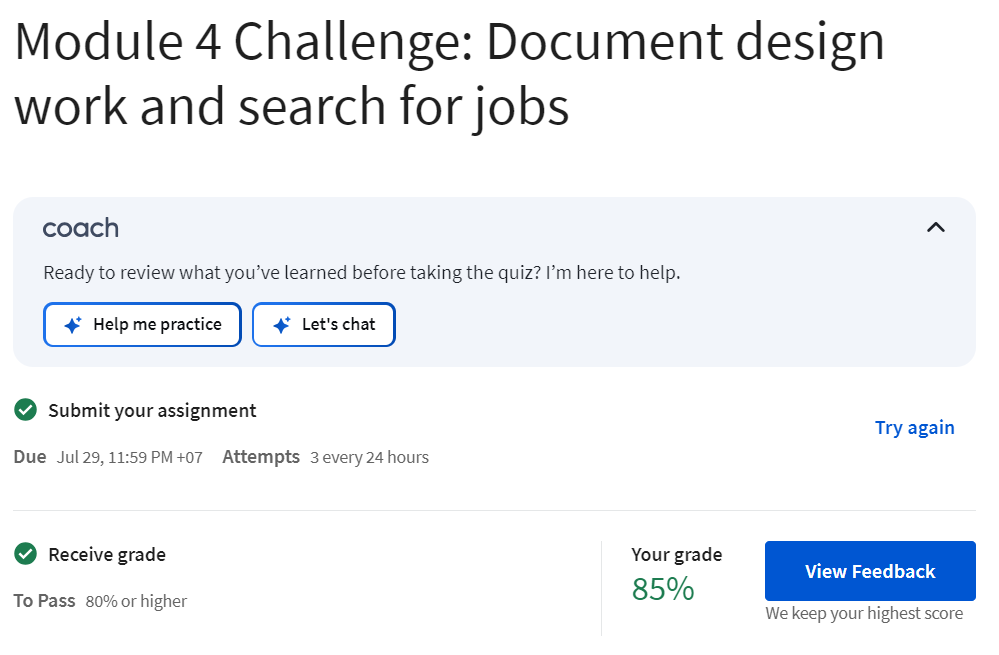
\includegraphics[width=\textwidth]{imgs/Course6-M4.png}
	\end{subfigure}
	\hfill
	\begin{subfigure}{0.75\textwidth}
		\centering
		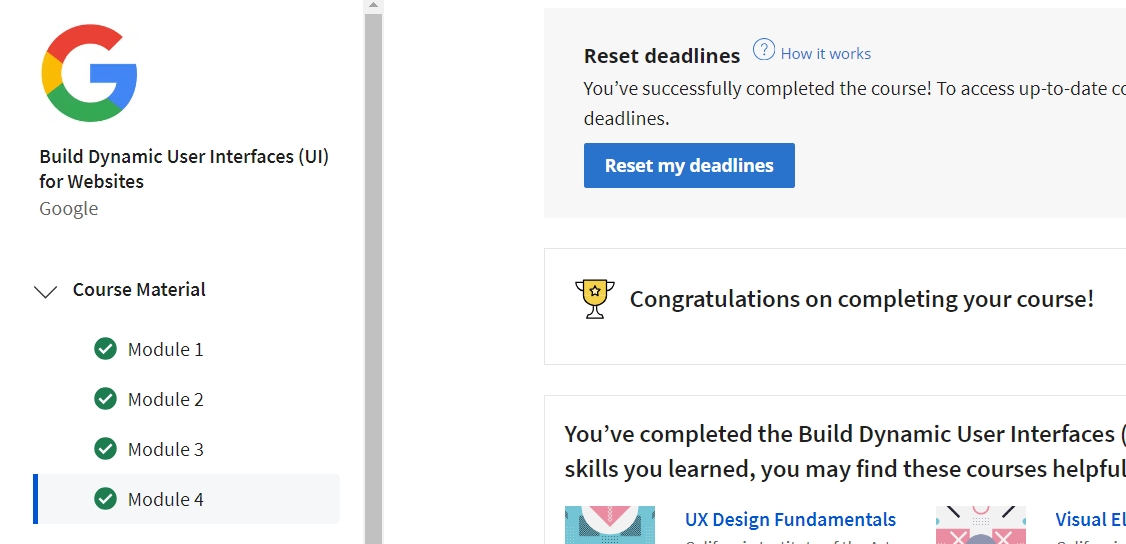
\includegraphics[width=\textwidth]{imgs/Course6-Done.png}
	\end{subfigure}
	\caption{Course 6 - Done}
\end{figure}

\subsubsection{Summary}
\begin{flushleft}
	What I have learned after completing this course:
	\begin{itemize}
		\item Apply each step of the UX design thinking framework (empathize, define, ideate, prototype, test) to create a dynamic website.
		\item Plan information architecture and sitemaps for website designs.
		\item Apply common layouts for web pages.
		\item Complete a design project and include it in your professional UX portfolio.
	\end{itemize}
\end{flushleft}

\subsubsection{Details}
\begin{flushleft}
	\begin{description}
		\item[Module 1:] Plan a responsive website
		      \begin{itemize}
			      \item I have completed the empathize and define phases.
		      \end{itemize}
		\item[Module 2:] Create and test prototypes
		      \begin{itemize}
			      \item I have learnt how to build a low-fidelity prototype.
			      \item I have made changes to my low-fidelity designs based on insights from my research.
		      \end{itemize}
		\item[Module 3:] Participating in design critique sections
		      \begin{itemize}
			      \item I have explored common website layouts, and created paper wireframes.
			      \item I have known a few elements and components that are commonly used in responsive website design.
			      \item I have updated and refined my wireframes to enhance accessibility.
		      \end{itemize}
		\item[Module 4:] Document design work and search for jobs
		      \begin{itemize}
			      \item I have learnt how to prepare and handoff designs to engineers, who will build the final product.
			      \item I have also added a case study to my professional UX portfolio featuring my responsive website designs.
			      \item I have learnt tips and tricks to scan job postings, and created a compelling resume that highlights my new UX skills.
		      \end{itemize}
	\end{description}
\end{flushleft}